\documentclass[../hw1.tex]{subfiles}

\begin{document}
    \sfsection{Summary and Self Test}
    \begin{enumerate}
        \inum{2}\item\ans{a, b, c} The stars we see at night depend on our location on Earth, Earth’s location in its orbit, and the time of the observation. The movement of stars through space is too slow for our eyes to see on Earth.
        \inum{7}\item\ans{b} If Earth’s axis had only a \ang{3} tilt, the seasons would be much less extreme. With a 3 degree tilt, over the course of a year there poles will point towards/away from the sun with only 3 degrees deviating from straight up and down.
        \ans{a}\item If you see the first quarter Moon overhead on the meridian, the Sun will be on the western horizon. During a first quarter Moon, the sun will be setting when the Moon is on the meridian and the sun sets in the west which means it will be on the western horizon.
        \inum{10}\item\ans{a, b, d} If the Moon were in the same orbital plane, but twice as far from Earth, total eclipses of the sun would not be possible, and the Moon’s cycle would take longer. At the moment where the Moon is barely allows for total eclipses of the sun and sometimes now when the moon is a little further from the Earth the Moon is not large enough to cover the Sun. With twice the diameter of orbit, the period of Moon's orbit would be longer and so the Moon's cycle would take longer. The phases of the moon, however, would be the same since the the moon will still orbit the Earth on the same plane and have one side lit on the moon. Earth's shadow will also still cover the Moon making lunar eclipses still possible.
    \end{enumerate}
    %\sfsection{Questions and Problems}
    \sfsection{Multiple Choice and True/False}
    \begin{enumerate}
        \inum{16}\item\ans{e} The tilt of Earth’s axis causes seasons because the days are longer in the summer and the rays of light strike the ground more directly in the summer.
        \inum{23}\item\ans{d} If you were standing at Earth’s South Pole, you would see no stars rising and setting. On the South Pole, as the Earth rotates, all the stars are circumpolar and no star will go past the horizon and come back. 
    \end{enumerate}

    \sfsection{Conceptual Questions}
    \begin{enumerate}
        \inum{29}\item The zodiacal constellations are associated with the times when that constellation is in the sun which will be during the day and not when the constellation is visible at night. As such, Sagittarius is associated with December where it is not visible because of the sunlight. That is why Sagittarius is visible in the summer and not the winter.
        \inum{34}\item The claim that the defendant could not see the pedestrian because the full Moon was casting long shadows across the street at midnight is not credible. At full Moon, the Moon is directly overhead at midnight and so the shadows should be short, not long. The only exception would be if the defendant was near the Arctic circle where the Moon never gets far up in the sky.
        \inum{36}\item We do not see a lunar eclipse each time the Moon is full because the the moon orbits the Earth on a different plane than the ecliptic plane. For there to be a lunar eclipse, there must be a new moon in a position where the planes intersect which happens about twice a year. The same logic applies for a solar eclipse, but is even stricter because of the relative size of the moon and the sun.
        \inum{40}\item If you just experienced the longest day of the year in the Northern Hemisphere and the shortest day in the Southern Hemisphere, then you are flying on a solstice around June 21. To explain it to the person next to me I would show them a drawing (fig1)*. Because of the Earth’s tilt, certain days happen to be longer or shorter depending on where the Earth is in its orbit. On that day, it happened to be the summer solstice in the Northern Hemisphere which meant it was the longest day of the year and the Earth was in a position where the north side was angled toward the Sun. Since the North side is angled toward the sun, the South side would be angled away and that would mean it would be the shortest day in the Southern Hemisphere.
        \inum{47}\item \begin{enumerate}
            \item Altitude of North Celestial Pole from our latitude is at \ang{47}, visible in the diagram.
            \item The angle along the meridian between the celestial equator and the local zenith is \ang{47}, the same as our latitude on Earth. The altitude of the Sun on the winter solstice is $43 - 23.5 = \ang{19.5}$. The altitude of the Sun on the summer solstice is $43 + 23.5 = \ang{66.5}$.
        \end{enumerate}
        \begin{center}
            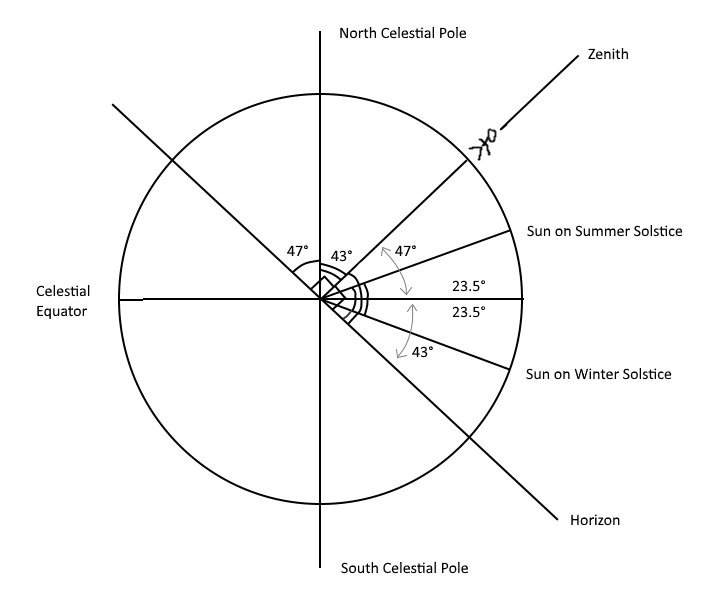
\includegraphics[scale=.65]{diagram}
        \end{center}
    \end{enumerate}

    \newpage
    \chead{Seasons}
    \sfsection{Seasons Homework}
        \onlyinsubfile{\subfile{seasonshw}}
        \notinsubfile{\subfile{assignments/seasonshw}}
    \sfsection{Moon Phases Homework}
        Moon Phases homework is attached with edits on the worksheet. There are minimal corrections.
\end{document}